\documentclass{article}
\usepackage[T1]{fontenc}
\usepackage{amsmath}
\usepackage{tikz}

\title{Week 10 Homework}

\begin{document}
\maketitle

\section*{Question 1}

\subsection*{(a)}

we are given:

\begin{itemize}
    \item metal sheet of thickness $d$ with mobile electron density $n$
    \item electrons displaced by $\Delta\ll d$ along the $x$ axis
\end{itemize}

displacing the electrons leaves a sheet of positive charge on one side and a sheet of negative charge on the other. each sheet has a thickness $\Delta$, so the charge per unit area is

\[
\sigma=ne\Delta
\]

the hint tells us to consider a small cylinder that encloses a piece of the positive sheet. by symmetry, the 
field points away from the sheet on both sides so the flux through the two ends is $2EA_c$ where $A_c$ is the 
end surface area of the cylinder. using Gauss' law,

\[
\oint E\cdot dA=\frac{Q_{\mathrm{enc}}}{\varepsilon_0}
\]
\[
2E_{+}A_c=\frac{\sigma A_c}{\varepsilon_0}
\]
\[
E_{+}=\frac{\sigma}{2\varepsilon_0}
\]

the negative sheet gives the same magnitude, so,

\[
E_{-}=\sigma/2\varepsilon_0
\]

between the two sheets, both fields point from the positive sheet towards the negative sheet, so they add

\[
E=E_{+}+E_{-}=\frac{\sigma}{\varepsilon_0}
\]

substituting $\sigma=ne\Delta$,

\[
\boxed{E=\frac{ne\Delta}{\varepsilon_0}}
\]

\subsection*{(b)}

once the electrons are released, each electron feels a force from the field. the field points 
from the positive sheet to the negative sheet, so the force on an electron points back towards equilibrium

\[
F=-eE=-\frac{ne^2\Delta}{\varepsilon_0}
\]

using $F=m_e\ddot{\Delta}$,

\[
m_e\ddot{\Delta}=-\frac{ne^2}{\varepsilon_0}\Delta
\]

\[
\boxed{\ddot{\Delta}+\frac{ne^2}{m_e\varepsilon_0}\Delta=0}
\]

this is the equation for undamped SHM.

\subsection*{(c)}

comparing with $\ddot{x}+\omega_0^2x=0$,

\[
\omega_0^2=\frac{ne^2}{m_e\varepsilon_0}
\]

\[
\boxed{\omega_0=\sqrt{\frac{ne^2}{m_e\varepsilon_0}}}
\]

\subsection*{(d)}

we are given:

\begin{itemize}
    \item density: $\rho=10.5\,\mathrm{g\,cm^{-3}}$
    \item atomic mass: $M=108\,\mathrm{g\,mol^{-1}}$
    \item one mobile electron per atom
\end{itemize}

since there is one mobile electron per atom, $n$ is the number density of atoms,

\[
n=\frac{\rho N_A}{M}
\]
\[
n=\frac{10.5}{108}(6.022\times10^{23})
\]
\[
n\approx5.85\times10^{22}\,\mathrm{cm^{-3}}=5.85\times10^{28}\,\mathrm{m^{-3}}
\]

substituting into the result from (c),

\[
\omega_0^2=\frac{(5.85\times10^{28})(1.602\times10^{-19})^2}
{(9.109\times10^{-31})(8.854\times10^{-12})}
\]
\[
\omega_0^2\approx1.86\times10^{32}\,\mathrm{s^{-2}}
\]
\[
\boxed{\omega_0\approx1.36\times10^{16}\,\mathrm{rad\,s^{-1}}}
\]

the frequency is

\[
f=\frac{\omega_0}{2\pi}\approx2.17\times10^{15}\,\mathrm{Hz}
\]

the wavelength of light with this frequency is

\[
\lambda=\frac{c}{f}=\frac{2\pi c}{\omega_0}
\]
\[
\lambda=\frac{2\pi(2.998\times10^{8})}{1.365\times10^{16}}
\]
\[
\lambda\approx1.38\times10^{-7}\,\mathrm{m}
\]

\[
\boxed{\lambda\approx138\,\mathrm{nm}}
\]

this is in the ultraviolet.

\section*{Question 2}

\subsection*{(a)}

we are given:

\begin{itemize}
    \item bridge height: $H=100\,\mathrm{m}$
    \item the cord stretches by $20\%$ when the jumper hangs from it
    \item the fall stops exactly at the river
\end{itemize}

let the unstretched length of the cord be $L$.

when the jumper hangs at rest, the spring force balances gravity and the extension is $0.2L$,

\[
k(0.2L)=mg
\]
\[
k=\frac{5mg}{L}
\]

at the lowest point the jumper is at the river, so the cord has been stretched by

\[
x_{\max}=H-L
\]

the jumper is at rest at the top and at the bottom, so all the gravitational potential energy lost goes into the elastic energy of the cord,

\[
mgH=\frac{1}{2}k(H-L)^2
\]

substituting $k=5mg/L$,

\[
mgH=\frac{5mg}{2L}(H-L)^2
\]
\[
100=\frac{5}{2L}(100-L)^2
\]
\[
40L=(100-L)^2
\]
\[
L^2-240L+10000=0
\]

using the quadratic formula,

\[
L=\frac{240\pm\sqrt{240^2-4(10000)}}{2}
\]
\[
L=\frac{240\pm\sqrt{17600}}{2}
\]
\[
L\approx53.7\,\mathrm{m}\quad\text{or}\quad L\approx186\,\mathrm{m}
\]

the cord cannot be longer than the bridge height, so we reject the second root,

\[
\boxed{L\approx53.7\,\mathrm{m}}
\]

\subsection*{(b)}

after the oscillations stop the jumper hangs at rest, where the cord is stretched by $20\%$,

\[
\text{extension}=0.2L\approx10.7\,\mathrm{m}
\]

so the total length of the hanging cord is

\[
1.2L\approx64.4\,\mathrm{m}
\]

the height above the river is

\[
h=H-1.2L
\]
\[
h=100-64.4
\]

\[
\boxed{h\approx35.6\,\mathrm{m}}
\]

\subsection*{(c)}

for small oscillations about the equilibrium position the cord stays taut, so the jumper behaves as a mass on a spring,

\[
\omega_0=\sqrt{\frac{k}{m}}
\]

the period is

\[
T=\frac{2\pi}{\omega_0}=2\pi\sqrt{\frac{m}{k}}
\]

using $k=5mg/L$,

\[
T=2\pi\sqrt{\frac{L}{5g}}
\]
\[
T=2\pi\sqrt{\frac{53.67}{5(9.81)}}
\]
\[
T\approx6.57\,\mathrm{s}
\]

\[
\boxed{T\approx6.6\,\mathrm{s}}
\]

\section*{Question 3}

\subsection*{(a)}

we are given:

\begin{itemize}
    \item resonant frequency: $f_0=19.7\,\mathrm{MHz}$
    \item mass: $m=9.7\times10^{-16}\,\mathrm{kg}$
    \item quality factor: $Q=40000$
\end{itemize}

the angular frequency is

\[
\omega_0=2\pi f_0
\]
\[
\omega_0=2\pi(19.7\times10^{6})
\]
\[
\omega_0\approx1.238\times10^{8}\,\mathrm{rad\,s^{-1}}
\]

since $\omega_0^2=k/m$,

\[
k=m\omega_0^2
\]
\[
k=(9.7\times10^{-16})(1.238\times10^{8})^2
\]
\[
\boxed{k\approx14.9\,\mathrm{N\,m^{-1}}}
\]

\subsection*{(b)}

the quality factor is

\[
Q=\frac{\omega_0}{\gamma}
\]

so,

\[
\gamma=\frac{\omega_0}{Q}
\]
\[
\gamma=\frac{1.238\times10^{8}}{40000}
\]
\[
\boxed{\gamma\approx3.09\times10^{3}\,\mathrm{s^{-1}}}
\]

\subsection*{(c)}

since $Q$ is large, we have $\omega_0/\gamma\gg10$, so we can use $\omega'\approx\omega_0$. the undriven motion is a decaying oscillation,

\[
x(t)\approx A_0e^{-\gamma t/2}\cos(\omega_0t)
\]

the energy of the oscillator is

\[
E=\frac{1}{2}kA^2
\]

and the amplitude decays as $A=A_0e^{-\gamma t/2}$, so

\[
E(t)=\frac{1}{2}kA_0^2e^{-\gamma t}
\]

differentiating,

\[
\frac{dE}{dt}=-\gamma E
\]

so,

\[
\boxed{\frac{dE}{dt}=-\frac{\gamma}{2}kA_0^2e^{-\gamma t}}
\]

at $t=0$ the energy is lost at a rate $\gamma E_0=\frac{1}{2}\gamma kA_0^2=\frac{1}{2}m\gamma\omega_0^2A_0^2$.

\subsection*{(d)}

on resonance $\omega=\omega_0$, so the steady state amplitude is

\[
A=\frac{F_0}{m\sqrt{(\omega_0^2-\omega^2)^2+\gamma^2\omega^2}}
\]
\[
A=\frac{F_0}{m\gamma\omega_0}
\]

rearranging for the driving force,

\[
F_0=m\gamma\omega_0A
\]

substituting, with $A=400\,\mathrm{fm}=4\times10^{-13}\,\mathrm{m}$,

\[
F_0=(9.7\times10^{-16})(3.09\times10^{3})(1.238\times10^{8})(4\times10^{-13})
\]

\[
\boxed{F_0\approx1.49\times10^{-16}\,\mathrm{N}}
\]

this is the same as $kA/Q$, as expected.

\subsection*{(e)}

the drive frequency is

\[
\omega=2\pi(19.7001\times10^{6})
\]

so the drive is above resonance, with

\[
\omega-\omega_0=2\pi(100)\approx628\,\mathrm{rad\,s^{-1}}
\]

the phase of the position relative to the drive is

\[
\phi=-\arg\left(\omega_0^2-\omega^2+i\gamma\omega\right)
\]

since $\omega\approx\omega_0$,

\[
\omega_0^2-\omega^2\approx-2\omega_0(\omega-\omega_0)
\]
\[
\omega_0^2-\omega^2\approx-2(1.238\times10^{8})(628)
\]
\[
\omega_0^2-\omega^2\approx-1.555\times10^{11}\,\mathrm{s^{-2}}
\]

and,

\[
\gamma\omega\approx(3.09\times10^{3})(1.238\times10^{8})
\]
\[
\gamma\omega\approx3.83\times10^{11}\,\mathrm{s^{-2}}
\]

the real part is negative and the imaginary part is positive, so the complex number lies in the second quadrant,

\[
\arg\left(\omega_0^2-\omega^2+i\gamma\omega\right)=\pi-\arctan\left(\frac{3.83}{1.555}\right)
\]
\[
\arg\left(\omega_0^2-\omega^2+i\gamma\omega\right)\approx1.957\,\mathrm{rad}
\]

hence,

\[
\boxed{\phi\approx-1.96\,\mathrm{rad}\approx-112^\circ}
\]

so the position lags the drive by about $112^\circ$.

the velocity is $\dot{x}=i\omega x$, so there is an extra phase of $\pi/2$ compared to the position,

\[
\theta=\phi+\frac{\pi}{2}
\]
\[
\theta\approx-1.957+1.571
\]

\[
\boxed{\theta\approx-0.39\,\mathrm{rad}\approx-22^\circ}
\]

so the velocity lags the drive by about $22^\circ$.

this agrees with the angles for $\omega>\omega_0$, where $-\pi<\phi<-\pi/2$ and $-\pi/2<\theta<0$.

\subsection*{(f)}

with honey, $\gamma=4\omega_0$, so

\[
\frac{\gamma}{2}=2\omega_0>\omega_0
\]

this is the over-damped case. the general solution is

\[
x(t)=C_1e^{\alpha_1t}+C_2e^{\alpha_2t}
\]

where

\[
\alpha_{1,2}=-\frac{\gamma}{2}\pm\sqrt{\left(\frac{\gamma}{2}\right)^2-\omega_0^2}
\]

substituting $\gamma=4\omega_0$,

\[
\alpha_{1,2}=-2\omega_0\pm\sqrt{4\omega_0^2-\omega_0^2}
\]
\[
\alpha_{1,2}=-2\omega_0\pm\sqrt{3}\,\omega_0
\]

so,

\[
\alpha_1=-(2-\sqrt{3})\omega_0\approx-0.268\omega_0
\]
\[
\alpha_2=-(2+\sqrt{3})\omega_0\approx-3.73\omega_0
\]

now we use the initial conditions, $x(0)=0$ and $\dot{x}(0)=v_0$.

\[
x(0)=C_1+C_2=0
\]
\[
C_2=-C_1
\]

\[
\dot{x}(0)=\alpha_1C_1+\alpha_2C_2=v_0
\]
\[
C_1(\alpha_1-\alpha_2)=v_0
\]

since $\alpha_1-\alpha_2=2\sqrt{3}\,\omega_0$,

\[
C_1=\frac{v_0}{2\sqrt{3}\,\omega_0}
\]

therefore,

\[
\boxed{x(t)=\frac{v_0}{2\sqrt{3}\,\omega_0}\left(e^{-(2-\sqrt{3})\omega_0t}-e^{-(2+\sqrt{3})\omega_0t}\right)}
\]

\subsection*{(g)}

for $t\gg1/\omega_0$ the term with $\alpha_2$ has already died away, since $|\alpha_2|>|\alpha_1|$. so only the slower term remains,

\[
x(t)\approx\frac{v_0}{2\sqrt{3}\,\omega_0}e^{-(2-\sqrt{3})\omega_0t}
\]

the decay rate of the amplitude is therefore

\[
\boxed{(2-\sqrt{3})\omega_0\approx0.268\omega_0\approx3.3\times10^{7}\,\mathrm{s^{-1}}}
\]

the energy, which goes as $x^2$, decays at twice this rate.

for comparison, without honey the amplitude decays at $\gamma/2\approx1.5\times10^{3}\,\mathrm{s^{-1}}$, so the honey makes the decay about $2\times10^{4}$ times faster.

\subsection*{(h)}

without honey, the resonator is under-damped, so the motion is an oscillation with period

\[
T=\frac{2\pi}{\omega_0}
\]

inside an envelope that decays slowly at rate $\gamma/2$.

with honey, the resonator is over-damped, so there is no oscillation. the position goes to a single maximum and then decays at rate $(2-\sqrt{3})\omega_0$, which is much faster than the decay without honey.

\bigskip
(just to mention, ai was NOT used to make this graph, i was having some fun :3)

\begin{center}
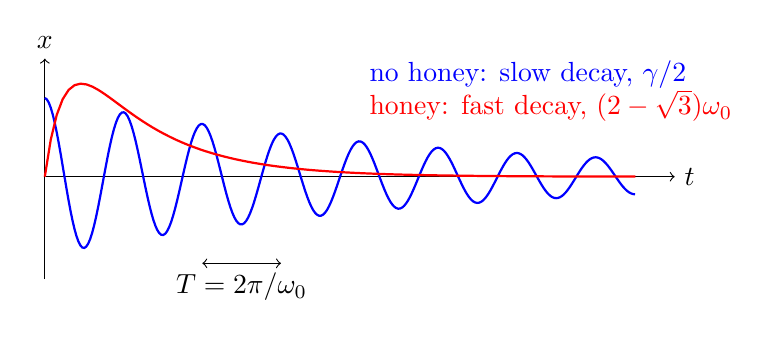
\begin{tikzpicture}
    \draw[->] (0,0) -- (8,0) node[right] {$t$};
    \draw[->] (0,-1.3) -- (0,1.5) node[above] {$x$};

    % without honey
    \draw[thick,blue,samples=300,domain=0:7.5]
        plot (\x,{exp(-0.2*\x)*cos(\x*360)});

    % with honey
    \draw[thick,red,samples=100,domain=0:7.5]
        plot (\x,{2.5*(exp(-1*\x)-exp(-4*\x))});

    % period
    \draw[<->] (2,-1.1) -- (3,-1.1) node[midway,below] {$T=2\pi/\omega_0$};

    \node[blue,anchor=west] at (4,1.3) {no honey: slow decay, $\gamma/2$};
    \node[red,anchor=west] at (4,0.9) {honey: fast decay, $(2-\sqrt{3})\omega_0$};
\end{tikzpicture}
\end{center}

the sketch is not to scale in time for the no honey envelope, since the real decay rates differ by a factor of about $2\times10^{4}$. the honey curve is drawn using the true ratio between $\omega_0$ and its decay rate.

\end{document}